\section{Алгоритм решения задачи и численные примеры}\label{sec:experiments}
Представим алгоритм решения задачи управления.
В соответствии с~\eqref{OC2} градиент функционала качества равен
\[
    J'_\lambda (u) = \lambda u - p_2.
\]
Здесь $u\in U$ -- управление в граничном условии~\eqref{bc1}, $p_2$ -- соответствующая компонента
сопряженного состояния из системы~\eqref{OC1}--\eqref{OC2}.

Предлагаемый алгоритм решения задачи (CP) выглядит следующим образом:
\begin{algorithm}[H]
    \caption{Алгоритм градиентного спуска}
    \begin{algorithmic}[1]
        \State Выбираем значение градиентного шага $\varepsilon$,
        \State Выбираем количество итераций $N$,
        \State Выбираем начальное приближение для управления $u_0 \in U$,
        \For{$k \gets 0,1,2,\dots,N$}
            :
            \State Для данного $u_k$ рассчитываем состояние $y_k = \{\theta_k, \varphi_k\}$ --
            решение задачи~\eqref{eq1},\eqref{bc1}.
            \State Рассчитываем значение функционала качества $J_\lambda(\theta_k, u_k)$.
            \State Рассчитываем сопряженное состояние $p_k=\{p_{1k},p_{2k}\}$ из уравнений~\eqref{OC1},
            где $ \hat{\theta} := \theta_k, \hat{u}=u_k$.
            \State Пересчитываем управление $u_{k+1} = u_k - \varepsilon (\lambda u_k - p_2)$
        \EndFor
    \end{algorithmic}
\end{algorithm}
Значение параметра $\varepsilon$ выбирается эмпирически таким образом, чтобы значение
$\varepsilon (\lambda u_k - p_2)$ являлось существенной поправкой для $u_{k+1}$.
Количество итераций $N$ выбирается достаточным для выполнения условия
$J_\lambda(\theta_k, u_k) - J_\lambda(\theta_{k+1}, u_{k+1}) < \delta$, где $\delta>0$ определяет точность расчетов.

Примеры, рассмотренные ниже, иллюстрируют работоспособность предложенного алгоритма при
малых значениях, что важно, параметра регуляризации $\lambda \leq 10^{-12}.$
В первом примере выполнены тестовые расчеты для куба.
Во втором примере приводится сравнение расчетов по
предложенному алгоритму с результатами работы~\cite{CNSNS19}.


Отметим, что для численного решения прямой задачи с заданным управлением использовалась слабая формулировка
и метод простой итерации для линеаризации задачи.
Решение сопряженной системы, которая является линейной при заданной температуре, не вызывает трудностей.
Для численного моделирования использовался солвер FEniCS~\cite{fenics, dolfin}.

\textbf{Пример 1.}
Приведем примеры расчетов для куба
$\Omega = {(x, y, z), 0 \leq x,y,z \leq l}$.
Будем считать, что $l=1~\text{см}$, $a = 0.006[\text{см}^2/\text{c}]$,
$b=0.025[\text{см}/\text{с}]$,
$\kappa_a=1[\text{см}^{-1}]$, $\alpha = 0.(3)[\text{см}]$.
Указанные параметры соответствуют стеклу~\cite{Grenkin5}.
Параметр регуляризации $\lambda=10^{-12}.$

Пусть граничные данные $r$ и $u$ в~\eqref{bc1} имеют вид:
\begin{gather*}
    r = 0.8 cos(\frac{\pi}{2}x) + 0.1,\quad
    u = \hat u = y.
\end{gather*}
Далее рассчитываем состояние $\theta$ и $\varphi$ как решение задачи~\eqref{eq1}--\eqref{bc1} и в качестве
$\theta_b$ выбираем граничные значение функции $\theta$ на $\Gamma$.
Значения нормальной производной $\partial_n\theta$ на $\Gamma$ должны соответствовать
значениям $q_b=r/a-\theta_b.$
Применяя предложенный алгоритм с начальным приближением $u_0 = 0.1$, находим приближенное решение
$\{\theta_\lambda,\varphi_\lambda,u_\lambda\}$ задачи (CP)\@.
Для демонстрации того, что алгоритм находит приближенное решение задачи с данными
Коши для температуры, важно сравнить значения $\partial_n\theta_\lambda$ на $\Gamma$ с $q_b.$

На рисунке~\ref{fig1:img_test_1} представлены изолинии модуля разности $|\partial_n\theta_\lambda-q_b|$
на грани куба в плоскости $z=l$, где $\partial_n\theta_\lambda=\partial\theta_\lambda/\partial z$, а также динамика функционала качества, определяющего
норму разности $\|\theta_\lambda -\theta_b\|^2_\Gamma$.
На остальных гранях куба значения $\partial_n\theta_\lambda-q_b$ имеют тот же порядок малости.

\begin{figure}[H]
    \centering
    \subfloat[$|q_n - \partial_n\theta|$]
    {
        \label{fig1:img_test_1}
        \includegraphics[width=.49\linewidth]{img/exp1/theta_n_diff_auto.png}
    }
    \subfloat[Изменение функционала в зависимости от числа итераций]
    {
        \label{fig1:quality}
        \includegraphics[width=.49\linewidth]{img/exp1/quality}
    }
    \caption{Результаты первого эксперимента}
    \label{fig1}
\end{figure}

\textbf{Пример 2.}
Сравним работу предложенного алгоритма с результатами статьи~\cite{CNSNS19}, где
соавтором был один из авторов данной работы.
Задача рассматривается в области $\Omega\times (-L,L)$, где $\Omega = \{ x = (x_1,x_2) \colon 0 < x_{1,2} < d\}$
и при больших $L$ сводится к двумерной задаче с вычислительной областью $\Omega$.
Выбраны следующие значения параметров задачи: $d= \mathrm{1(m)}$, $a = 0.92~10^{-4}~\mathrm{(m^2/s)}$, $b=
0.19~\mathrm{(m/s)}$, $\alpha = 0.0333~\mathrm{(m)}$ и $\kappa_a = 1~\mathrm{(m^{-1})}$.
Параметры соответствуют воздуху при нормальном атмосферном давлении и температуре 400$^\circ$C\@.

Функции $\theta_b$, $q_b$ в краевом условии~\eqref{bc2} заданы следующим образом:
$\theta_b = \widehat{\theta}|_{\Gamma}$, $q_b = \partial_n \widehat{\theta}|_{\Gamma}$, где
$\widehat{\theta} = (x_1-0.5)^2 - 0.5x_2+0.75$.

Приближенное решение задачи с данными Коши, представленное в~\cite{CNSNS19} (рис.~\ref{fig2:CNSNS19}),
получено путем решения эллиптической задачи четвертого
порядка для температуры методом установления по времени.
Использовались $H^2$ конформные конечные элементы Богнера-Фокса-Шмитта и
солвер FeliCs, разработанный в техническом университете Мюнхена.
Решение стабилизировалось через 120 секунд, но вычисления на каждом временном
шаге потребовали довольно значительных затрат.

На рис.~\ref{fig2:theta_auto} отображено температурное поле, полученное
предложенным в данной статье методом.
На рис.~\ref{fig:theta_n} приведёны графики функций
$q_b, \partial_n \theta_{init}, \partial_n \theta_{end}$ на $\Gamma$, где $\theta_{init}$ есть решение прямой
задачи на нулевой итерации, $\theta_{end}$ на последней.
На рис.~\ref{fig3:quality} приведена динамика функционала качества по итерациям.


Как видно из представленных рисунков, предложенный алгоритм достаточно успешно справляется
с получением приближенного решения для задачи~\eqref{eq1}--\eqref{bc1}.

Исходный код расчётов, а также инструментарий по отрисовке графиков можно найти по ссылке~\cite{mesenev-github}.

\begin{figure}[H]
    \centering
    \subfloat[Температурное поле, полученное в статье~\cite{CNSNS19}]
    {
        \label{fig2:CNSNS19}
        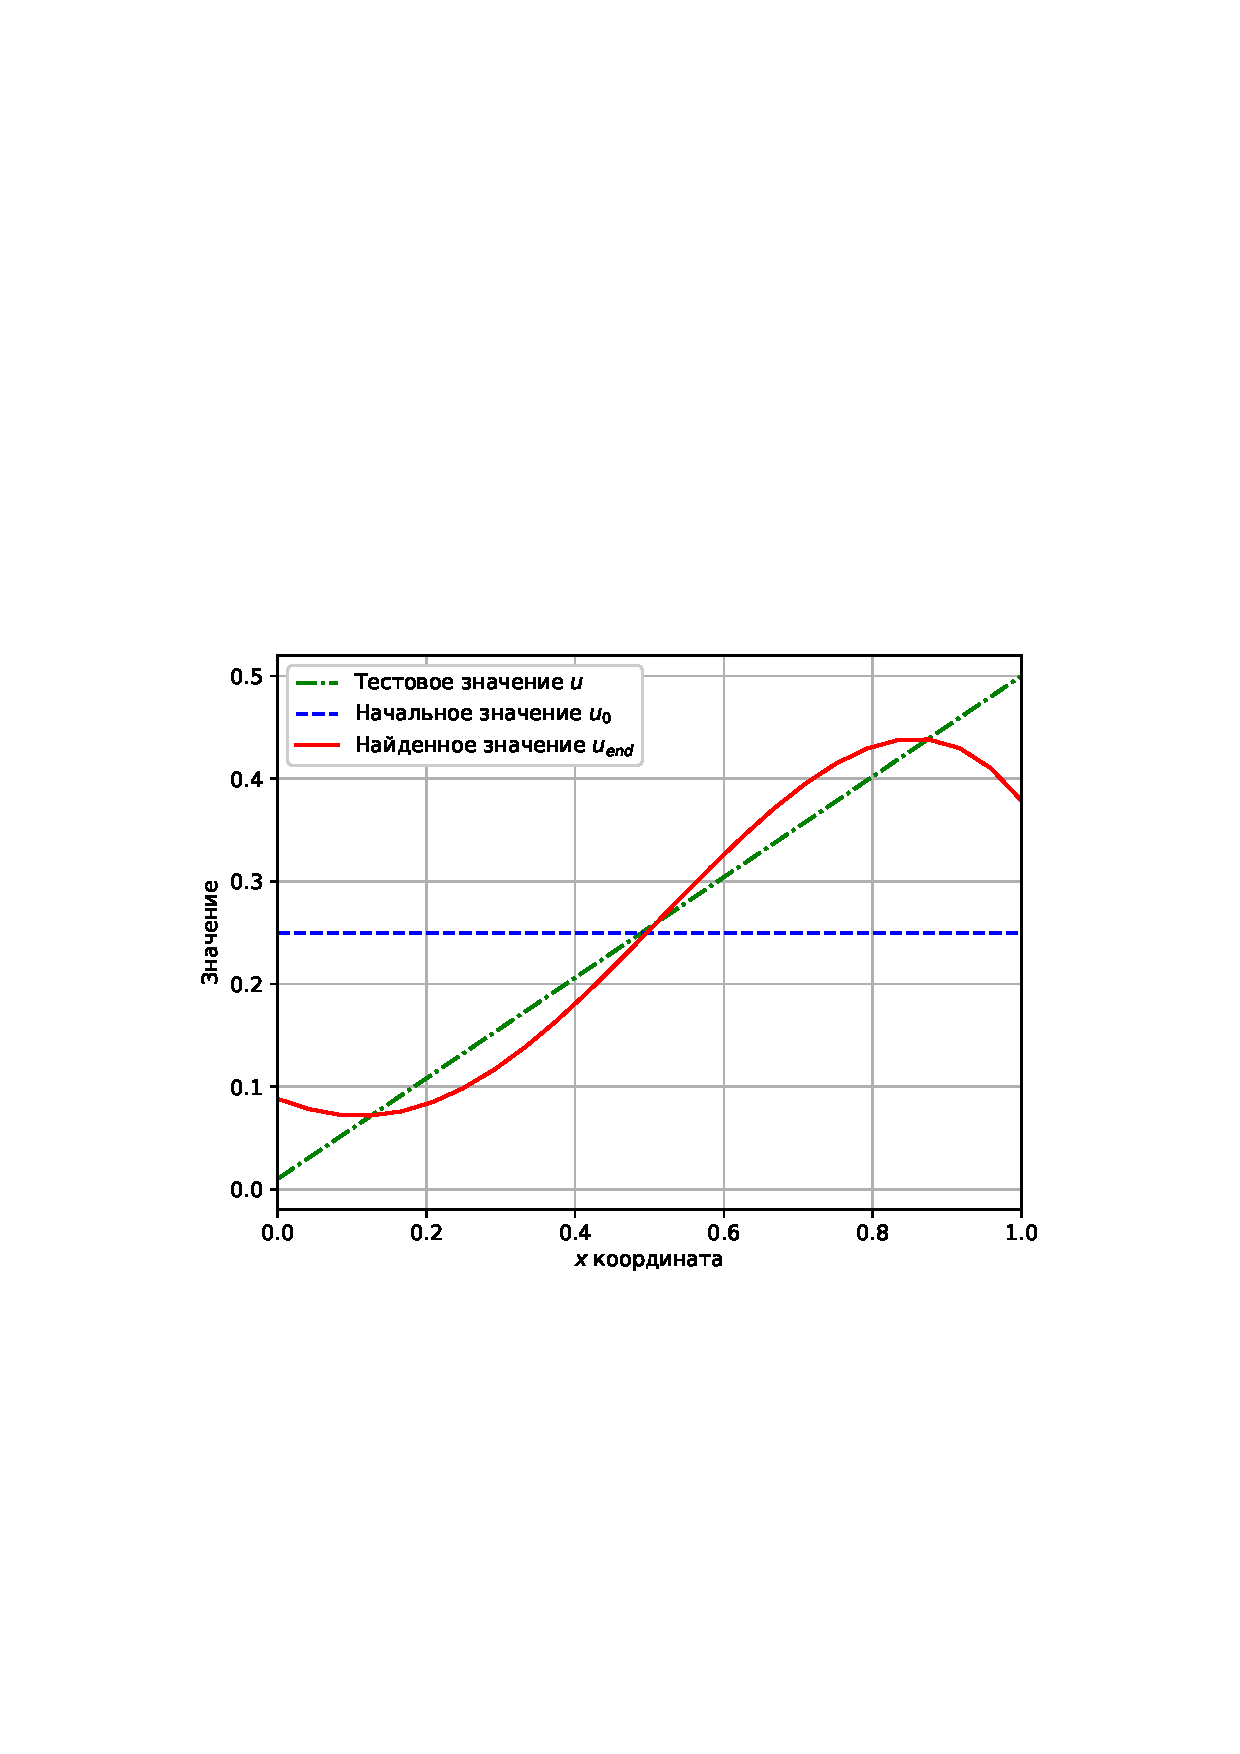
\includegraphics[width=.49\linewidth]{img/exp2/2.jpeg}
    }
    \subfloat[Температурное поле, полученное предложенным алгоритмом]
    {
        \label{fig2:theta_auto}
        \includegraphics[width=.49\linewidth]{img/exp2/theta.png}
    }
    \caption{Графики температурного поля $\theta$}
    \label{fig2}
\end{figure}

\begin{figure}[H]
    \centering
    \subfloat[График функций $q_b, \partial_n \theta_{init}, \partial_n \theta_{end}$]
        {
        \label{fig:theta_n}
        \includegraphics[width=.49\linewidth]{img/exp2/theta_n_g}
    }
    \subfloat[Изменение функционала качества]
    {
        \label{fig3:quality}
        \includegraphics[width=.49\linewidth]{img/exp2/quality}
    }
    \caption{}
    \label{fig3}
\end{figure}
